%SourceDoc ws-skript.tex
%
% c04-verteilung.tex
%
% (c) 2006 Prof. Dr. Andreas M�ller
% $Id: c04a-verteilung.tex,v 1.17 2008/09/09 14:22:16 afm Exp $
%
\rhead{Verteilungen}
\chapter{Ein Katalog von Wahrscheinlichkeitsverteilungen
\label{chapter-wahrscheinlichkeitsverteilung-katalog}}
Im Laufe der Zeit ist eine grosse Zahl von Verteilungen gefunden worden,
die die verschiedensten von Zufalls beeinflussten Prozesse in der realen
Welt beschreiben. In diesem Kapitel werden einge praktisch wichtige
Verteilungen vorgestellt.
\section{Stetige Wahrscheinlichkeitsverteilungen}

\subsection{Gleichverteilung\label{section-gleichverteilung-stetig}}
\begin{table}
\renewcommand{\arraystretch}{1.5}
\begin{center}
\begin{tabular}{|l|l|}
\hline
Name&Gleichverteilung\\
\hline
Dichtefunktion&
\begin{minipage}{3.7in}
\vskip5pt
$\displaystyle
\begin{cases}
\frac1{b-a}&\qquad a\le x\le b\\
0&\qquad\text{sonst}
\end{cases}
$
\end{minipage}
\\[8pt]
Verteilungsfunktion&
\begin{minipage}{3.7in}
\vskip5pt
$\displaystyle
\begin{cases}0&\qquad x\le a\\
\frac{x-a}{b-a}&\qquad x \le a \le b\\
1&\qquad x>b\end{cases}
$
\end{minipage}
\\[8pt]
Erwartungswert&
\begin{minipage}{3.7in}
\vskip3pt
$\displaystyle \frac{a+b}2$
\end{minipage}
\\[8pt]
Varianz&
\begin{minipage}{3.7in}
\vskip3pt
$\displaystyle \frac{(b-a)^2}{12}$
\end{minipage}
\\[8pt]
Median&
\begin{minipage}{3.7in}
\vskip3pt
$\displaystyle \frac{a+b}{2}$
\end{minipage}
\\[8pt]
$P(|X-E(X)|>\varepsilon)$&
\begin{minipage}{3.7in}
\vskip3pt
$\displaystyle 1-\frac{2\varepsilon}{b-a}$ f"ur $\varepsilon<\frac{b-a}2$
\end{minipage}
\\[10pt]
\hline
Anwendungen&\begin{minipage}{3.7in}%
\strut
$\bullet$ Verteilung von Zufallszahlen
\strut
\end{minipage}\\
\hline
\end{tabular}
\end{center}
\caption{Datenblatt der Gleichverteilung\label{datenblatt:gleichverteilung}}
\end{table}

\begin{figure}
\begin{center}
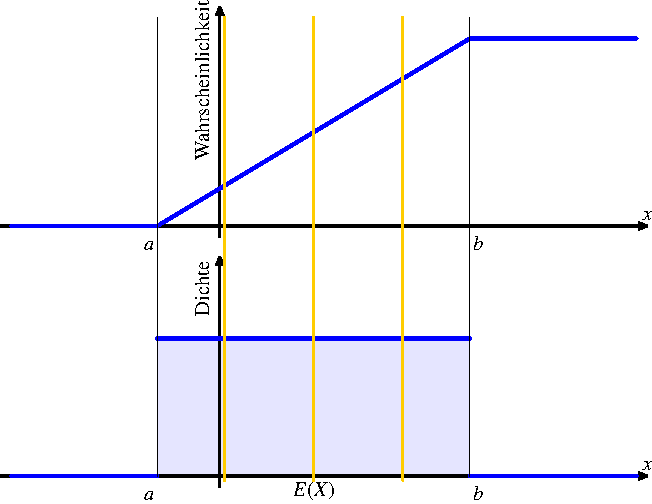
\includegraphics[width=0.8\hsize]{images/verteilungsfunktion-7}
\end{center}
\caption{Verteilungsfunktion (oben) und Wahrscheinlichkeitsdichte (unten)
der Gleichverteilung\label{bild-gleichverteilung}}
\end{figure}
\begin{figure}
\begin{center}
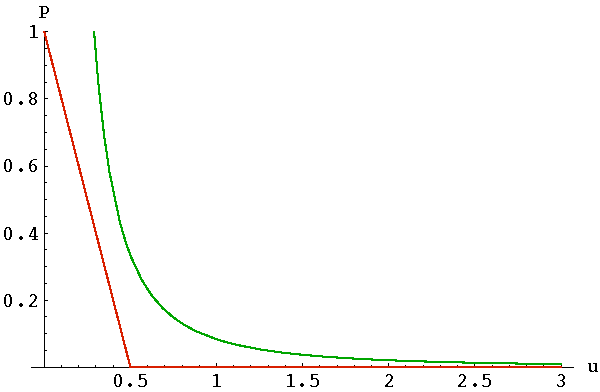
\includegraphics[width=0.8\hsize]{graphics/abwgl}
\end{center}
\caption{Wahrscheinlichkeit einer Abweichung vom Mittelwert einer
in $[0,1]$ gleichverteilten Zufallsvariable (rot) im Vergleich mit
der oberen Schranke aus dem Satz von Tschebyscheff (gr"un)
\label{bild-gleichverteilung}}
\end{figure}
Gleichverteilung der Werte einer Zufallsvariablen liegt vor, wenn
die Wahrscheinlichkeit, dass ein Wert in ein bestimmtes Intervall
f"allt, der L"ange des Intervalles proportional ist. Dies bedeutet,
dass die Verteilungsfunktion $F$ konstante Steigung hat. Da $0\le F(x)\le 1$
gelten muss, ist dies nur innerhalb eines Intervalls $[a,b]$ m"oglich.
\begin{definition}Die Zufallsvariable $X$ heisst auf dem Intervall
$[a,b]$ gleichverteilt, wenn sie die Verteilungsfunktion
\[
F(x)=\begin{cases}
0&\qquad x< a\\
\frac{x-a}{b-a}&\qquad x\in[a,b]\\
1&\qquad x> b
\end{cases}
\]
mit der Wahrscheinlichkeitsdichte
\[
\varphi(x)=\begin{cases}
0&\qquad x< a\\
\frac1{b-a}&\qquad x\in[a,b]\\
0&\qquad x> b
\end{cases}
\]
hat.
\end{definition}

\subsubsection{Erwartungswert und Varianz}
\begin{satz}Sei $X$ eine in $[a,b]$ gleichverteilte Zufallsvariable,
dann gilt
\begin{align*}
E(X)&=\frac{a+b}2\\
\operatorname{var}(X)&=\frac{(b-a)^2}{12}
\end{align*}
\end{satz}
\begin{proof}[Beweis]
Mit Hilfe der Dichtefunktion berechnet man den Erwartungswert
\begin{align*}
E(X)&=\int_{-\infty}^\infty \varphi(x)x\,dx=\int_a^b\frac{x}{b-a}\,dx\\
&=\frac1{b-a}\left[\frac12x^2\right]_a^b=\frac{b^2-a^2}{2(b-a)}=\frac{a+b}2
\end{align*}
und die Varianz
\begin{align*}
E(X^2)=&\int_{-\infty}^\infty x^2\varphi(x)\,dx=\frac1{b-a}\int_a^bx^2\,dx\\
&=\frac1{b-a}\left[\frac{x^3}3\right]_a^b=\frac{b^3-a^3}{3(b-a)}=\frac{a^2+ab+b^2}3\\
\operatorname{var}(X)&=\frac{a^2+ab+b^2}3-\frac{(b+a)^2}4\\
&=\frac{4a^2+4ab+4b^2-3b^2-6ab-3a^2}{12}\\
&=\frac{a^2-2ab+b^2}{12}=\frac13\left(\frac{b-a}2\right)^2\\
\sqrt{\operatorname{var}(X)}&=\frac1{\sqrt{3}}\cdot\frac{b-a}2\simeq 0.57\cdot\frac{b-a}2.
\end{align*}

\end{proof}

\subsubsection{*Wahrscheinlichkeit einer grossen Abweichung}
{\small
F"ur $\varepsilon>\frac{b-a}2$ ist die Wahrscheinlichkeit
$P(|X-\mu|>\varepsilon)$
einer Abweichung vom Erwartungswert $\mu=E(X)$ nat"urlich $0$,
aber f"ur kleinere $\varepsilon$ ergibt sich
\begin{eqnarray*}
P(|X-\mu|>\varepsilon)
&=&1-\int_{\mu-\varepsilon}^{\mu+\varepsilon}\varphi(x)\,dx
=1-\int_{\mu-\varepsilon}^{\mu+\varepsilon}\frac{1}{b-a}\,dx\\
&=&1-\frac1{b-a}\left[x\right]_{\mu-\varepsilon}^{\mu+\varepsilon}=1-\frac{2\varepsilon}{b-a}
\end{eqnarray*}
}

%\begin{table}
%\begin{center}
%\begin{tabular}{|l|l|}
%\hline
%Name&\\
%\hline
%Dichtefunktion&$\displaystyle$\\
%Verteilungsfunktion&$\displaystyle$\\
%Erwartungswert&$\displaystyle$\\
%Varianz&$\displaystyle $\\
%Median&$\displaystyle $\\
%$P(|X-E(X)|>\varepsilon)$&$\displaystyle $ \\
%\hline
%Anwendungen&\begin{minipage}{3.7in}%
%$\bullet$ \\
%$\bullet$ 
%\end{minipage}\\
%\hline
%\end{tabular}
%\end{center}
%\caption{Datenblatt der XXXverteilung\label{datenblatt:XXXverteilung}}
%\end{table}

\subsection{Exponentialverteilung\label{section-exponentialverteilung}}
\begin{table}
\renewcommand{\arraystretch}{2}
\begin{center}
\begin{tabular}{|l|l|}
\hline
Name&Exponentialverteilung\\
\hline
Dichtefunktion&$\displaystyle ae^{-ax}$\\
Verteilungsfunktion&$1-e^{-ax}$\\
Erwartungswert&$\displaystyle \frac1a$\\
Varianz&$\displaystyle \frac1{a^2}$\\
Median&$\displaystyle \frac1a\log 2$\\[8pt]
$P(|X-E(X)|>\varepsilon)$&
\begin{minipage}{3.7in}
$
\begin{cases}
e^{-a\varepsilon-1}&\qquad\text{f"ur $\varepsilon > \frac1a$}\\
1-e^{a\varepsilon-1}+e^{-a\varepsilon-1}&\qquad\text{f"ur $\varepsilon \le \frac1a$}
\end{cases}
$
\end{minipage}
\\[10pt]
\hline
Anwendungen&\begin{minipage}{3.7in}%
\strut
$\bullet$ Prozess ohne Erinnerungsverm"ogen\\
$\bullet$ Radioaktivit"at
\strut
\end{minipage}\\
\hline
\end{tabular}
\end{center}
\caption{Datenblatt der Exponentialverteilung\label{datenblatt:exponentialverteilung}}
\end{table}
\begin{figure}
\begin{center}
%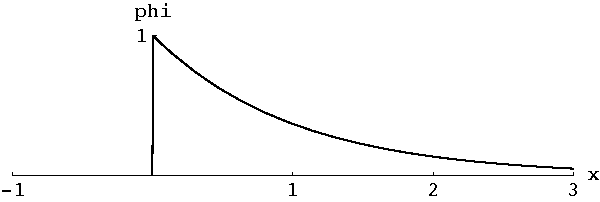
\includegraphics[width=0.8\hsize]{graphics/expphi}
%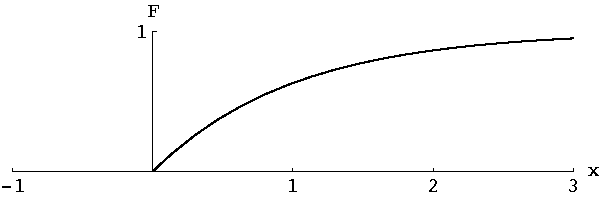
\includegraphics[width=0.8\hsize]{graphics/expF}
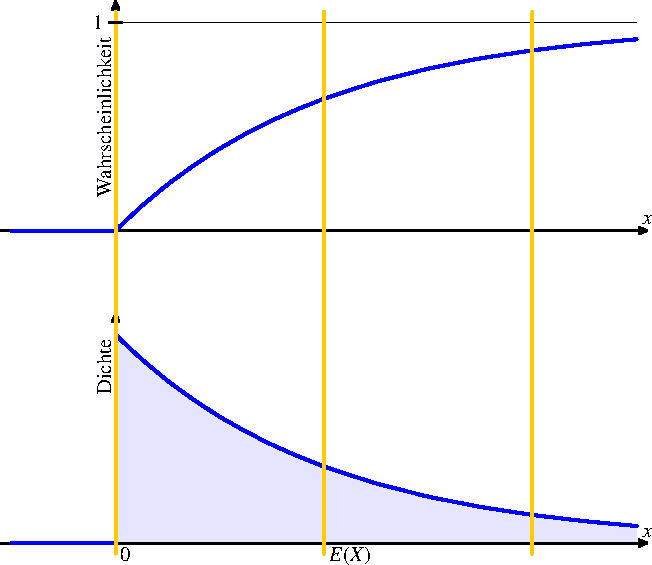
\includegraphics[width=0.8\hsize]{images/verteilungsfunktion-8}
\end{center}
\caption{Dichtefunktion (oben) und Verteilungsfunktion (unten) der Exponentialverteilung
\label{bildexponentialverteilung}}
\end{figure}
Bei radioaktiven Stoffen und bei gewissen Bauteilen stellt man fest,
dass ihr Zerfall bzw.~ihr Versagen kein Ged"achtnis hat.
Die Wahrscheinlichkeit, dass ein Atomkern innerhalb der Zeit $t$ zerf"allt,
ist gleich gross wie die Wahrscheinlichkeit, dass er zwischen $t_0$
und $t_0+t$ zerf"allt, wenn er bis zur Zeit $t_0$ nicht zerfallen ist.
Auch Bauteile ohne Erm"udungserscheinungen verhalten sich so.

\subsubsection{Verteilungsfunktion und Dichtefunktion}
Etwas formaler sei $X$ eine Zufallsvariable, die die Zeit angibt, zu der
ein Atomkern zerf"allt. Die ``Ged"achtnislosigkeit'' bedeutet, dass die
bedingte Wahrscheinlichkeit f"ur einen Zerfall vor $t_0+t$ unter der
Annahme, dass der Kern bis zur Zeit $t_0$ nicht zerfallen ist, gleich
gross ist wie die Wahrscheinlichkeit eines Zerfalls bis zur Zeit $t$:
\[
P(X \le t) = P(X\le t_0+t|X > t_0)
\]
Dies ist nat"urlich gleichbedeutend mit der Wahrscheinlichkeit f"ur
die negierten Ereignisse:
\[
P(X > t) = P(X > t_0+t|X > t_0)
\]
Aus der Definition der bedingten Wahrscheinlichkeit
\ref{def-bedingte-wahrscheinlichkeit} folgt
\[
P(X> t_0+t|X>t_0)=\frac{P(X>t_0+t\wedge X>t_0)}{P(X > t_0)}
=\frac{P(X>t_0+t)}{P(X>t_0)}
\]
Die Bedingung an die Verteilung wird damit zu
\[
P(X>t)P(X>t_0)=P(X>t+t_0).
\]
Schreiben wir jetzt $g(t)=P(X>t)=1-F(t)$, werden die Formeln
etwas "ubersichtlicher:
\[
g(t)g(t_0)=g(t+t_0).
\]
Zun"achst leiten wir nach $t_0$ ab, wir nehmen ja an, dass wir
eine stetige Zufallsvariable haben, und dass die Verteilungsfunktion
differenzierbar sein wird.
Wir erhalten
\[
g(t)g'(t_0)=g'(t+t_0).
\]
Jetzt lassen wir $t_0$ gegen $0$ streben, und bekommen
die Differentialgleichung
\[
g'(t)=g'(0)g(t)
\]
f"ur $g(t)$.
Diese lineare Differentialgleichung erster Ordnung
muss als L"osung eine Exponentialfunktion haben. Da $F(t)$
monoton w"achst, muss $g(t)$ monoton fallen, ausserdem
muss $g(t)$ beschr"ankt bleiben. Damit bleibt nur
$g(t)=e^{-at}$ mit einem positiven $a$.

\begin{definition}
Die Wahrscheinlichkeitsverteilung mit Dichtefunktion
\[
\varphi(x)=\begin{cases}
0&\qquad x<0\\
a e^{-a x}&\qquad x\ge 0
\end{cases}
\]
heisst Exponentialverteilung. Ihre Verteilungsfunktion ist
\[
F(x)=\begin{cases}
0&\qquad\text{f"ur $x < 0$}\\
1-e^{-ax}&\qquad\text{f"ur $x\ge 0$}.
\end{cases}
\]
\end{definition}
\index{Exponentialverteilung}
\index{Verteilungsfunktion!Exponentialverteilung}
\index{Wahrscheinlichkeitsdichte!Exponentialverteilung}
Wir sollten noch nachrechnen, dass dies tats"achlich die richtige
Verteilungsfunktion ist. Zun"achst w"achst sie tats"achlich monoton,
und auch der Grenzwert f"ur $t\to\infty$ ist wie gew"unscht. Aber
auch die Ableitung ist richtig:
\[
\frac{d}{dt}(1-e^{-at})=ae^{-at}\qquad\text{f"ur}\quad t>0.
\]

\subsubsection{Erwartungswert und Varianz}
\index{Erwartungswert!der Exponentialverteilung}
\index{Exponentialverteilung!Erwartungswert}
\index{Varianz!der Exponentialverteilung}
\index{Exponentialverteilung!Varianz}
\begin{satz}Eine exponentialverteilte Zufallsvariable $X$ mit Parameter
$a$ hat folgenden Erwartungswert und folgene Varianz:
\begin{eqnarray*}
E(X)&=&\frac1a\\
\operatorname{var}(X)&=&\frac1{a^2}
\end{eqnarray*}
\end{satz}
\begin{proof}[Beweis]
Zur Berechnung von Erwartungswert und Varianz ist es n"utzlich die Integrale
$I_n=\int \xi^ne^{-\xi}\,d\xi$
berechnen zu k"onnen. Diese findet man rekursiv durch partielle Integration:
\begin{eqnarray*}
I_n&=&\int \xi^ne^{-\xi}\,d\xi\\
&=&-\xi^ne^{-\xi}+n\int \xi^{n-1}e^{-\xi}\,d\xi\\
&=&-\xi^ne^{-\xi}+nI_{n-1}
\end{eqnarray*}
Um Erwartungswert und Varianz zu berechnen, verwendet man mit Vorteil die
Variablentransformation $ax=\xi$. F"ur den Erwartungswert ergibt sich:
\begin{align*}
E(X)&=\int_0^{\infty}ae^{-ax}x\,dx
=\frac1a\int_0^{\infty}ax e^{-ax}a\,dx
=\frac1a\int_0^{\infty}\xi e^{-\xi}\,d\xi\\
&=\frac1a\left[-\xi e^{-\xi}-e^{-\xi}\right]_0^\infty=\frac1a
\end{align*}
Analog f"ur die Varianz:
\begin{align*}
E(X^2)
&=
\int_0^{\infty}x^2ae^{-ax}\,dx
=\frac1{a^2}\int_0^{\infty}(ax)^2e^{-ax}a\,dx\\
&=\frac1{a^2}\int_0^{\infty}\xi^2e^{-\xi}\,d\xi
=\frac1{a^2}\left[\xi^2e^{-\xi}-2\xi e^{-\xi}+2e^{-\xi}\right]_0^\infty
=\frac2{a^2}
\\
\operatorname{var}(X)
&=E(X^2)-E(X)^2=\frac2{a^2}-\left(\frac1a\right)^2=\frac1{a^2}
\end{align*}
\end{proof}
Die Gr"osse $\frac1a$ l"asst sich also leicht interpretiren: sie ist die
mittlere ``Lebensdauer'', man findet sie oft unter dem K"urzel MTBF f"ur
mean time between failure.
Und $\sqrt{\operatorname{var}(X)}$ 
ist genau gleich gross. 
\index{Mean time between failure}
\index{MTBF}
\subsubsection{*Wahrscheinlichkeit grosser Abweichungen}
{
\small
\begin{figure}
\begin{center}
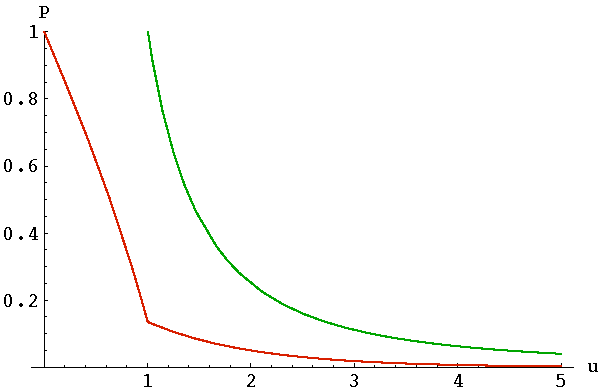
\includegraphics[width=0.8\hsize]{graphics/abwexp}
\end{center}
\caption{Wahrscheinlichkeit f"ur eine grosse Abweichung bei einer
Exponentialverteilten Zufallsvariable, oben die durch den Satz von Tschebyscheff egebene Schranke (gr"un), unten die exakte Rechnung mit
Hilfe der Exponentialvereteilung (rot)\label{abweichung-exponential}}
\end{figure}
Wir k"onnen nun auch die Wahrscheinlichkeit einer grossen Abweichung
berechnen:
\begin{satz} F"ur eine exponentialverteilte Zufallsvariable mit
Erwartungswert $\frac1a$ ist die Wahscheinlichkeit einer Abweichung
$\varepsilon$ vom Erwartungswert
\[
P(|X-{\textstyle\frac1a}|>\varepsilon)=
\begin{cases}
e^{-a\varepsilon-1}&\qquad\text{f"ur $\varepsilon > \frac1a$}\\
1-e^{a\varepsilon-1}+e^{-a\varepsilon-1}&\qquad\text{f"ur $\varepsilon \le \frac1a$}
\end{cases}
\]
\end{satz}
\begin{proof}[Beweis]
Die Wahrscheinlichkeit einer grossen Abweichung ist
\begin{eqnarray*}
P(|X-{\textstyle\frac1a}|>\varepsilon)
&=&1-\int_{\frac1a-\varepsilon}^{\frac1a+\varepsilon}\varphi_a(x)\,dx\\
&=&1-\int_{\max(0,\frac1a-\varepsilon)}^{\frac1a+\varepsilon}ae^{-ax}\,dx\\
&=&1-\left[-e^{-ax}\right]_{\max(0,\frac1a-\varepsilon)}^{\frac1a+\varepsilon}\\
&=&1+e^{-a\varepsilon-1}-e^{-\max(0,1-a\varepsilon)}\\
&=&\begin{cases}
e^{-a\varepsilon-1}&\qquad\text{f"ur $\varepsilon > \frac1a$}\\
1-e^{a\varepsilon-1}+e^{-a\varepsilon-1}&\qquad\text{f"ur $\varepsilon \le \frac1a$}
\end{cases}
\end{eqnarray*}
\end{proof}
Der Satz von Tschebyscheff setzt diese Wahrscheinlichkeit in Relation
zur Varianz
\[
P(|X-{\textstyle\frac1a}|>\varepsilon)\le
\frac{\operatorname{var}(X)}{\varepsilon^2}=\frac{1}{a^2\varepsilon^2},
\]
selbstverst"andlich muss diese Ungleichung immer noch erf"ullt sein.
Also
\begin{alignat*}{3}
e^{-a\varepsilon-1}&\le&\frac1{a^2\varepsilon^2}&\qquad\text{f"ur $a\varepsilon>1$}\\
1-e^{a\varepsilon-1}+e^{-a\varepsilon-1}&\le&\frac1{a^2\varepsilon^2}&\qquad\text{f"ur $a\varepsilon\le1$}
\end{alignat*}
In allen Ausdr"ucken kommt immer nur das Produkt $a\varepsilon$ vor,
wir k"onnen daher
abk"urzend $u=a\varepsilon$ schreiben. Die zweite Ungleichung wird dann zu
\[
\frac{1-e^{u}+e^{-u}}e\le\frac1{u^2}\qquad\text{f"ur $u\le1$}
\]
In diesem Fall ist die rechte Seite mindestens 1,
die Tschebyscheff-Ungleichung wird jetzt v"ollig nichtssagend, denn 
gr"osser als 1 kann die Wahrscheinlichkeit f"ur eine Abweichung ohnehin
nicht werden.

Die erste Ungleichung wird zu
\[
e^{-u-1}\le\frac1{u^2}\qquad\text{f"ur $u > 1$}.
\]
Diese Funktion f"allt monoton sehr schnell gegen 0, viel schneller
als der Ausdruck $\frac1{u^2}$. In der Abbildung~\ref{abweichung-exponential}
sieht man beide Schranken, die allgemeine, gegeben durch den
Satz von Tschebyscheff, und die exakte f"ur die Exponentialverteilung.
}

\subsubsection{Anwendung}
Ger"ate aller Art versuchen, die Lebensdauer dadurch zu erh"ohen, dass
kritische Komponenten redundant aufgebaut werden.
Zum Beispiel verwenden Server h"aufig zwei Disks, deren Daten
gespiegelt sind, so dass der Ausfall eines Disks noch keinen Ausfall
des Gesamtsystems verursacht. Wir wollen die erwartete Zeit bis zum
Ausfall des Gesamtsystems berechnen, wenn zwei Disks verwendet werden,
deren Zeit bis zum Ausfall exponentialverteilt ist. Weiter nehmen
wir an, dass die Disks unabh"angig voneinander ausfallen.

Sei also $X_i$ die Zeit bis zum Ausfall von Disk $i$, mit
Verteilungsfunktion $F_{X_i}(t)=1-e^{at}$ f"ur $t\ge 0$. Gesucht
ist die Verteilungsfunktion f"ur die Zeit $X$ bis zum Ausfall
des Gesamtsystems, also die Funktion $F(t)=P(X\le t)$. Das Gesamtsystem
f"allt aus, wenn beide Disks ausgefallen sind, es ist also
\begin{align*}
F(t)
&=P(X\le t)=P(X_1\le t\wedge X_2\le t)\\
&=P(X_1\le t)\cdot P(X_2\le t)
= F_{X_1}(t) F_{X_2}(t)=(1-e^{-at})^2
\end{align*}
Zur Berechnung des Erwartungswertes von $X$ wird die
Wahrscheinlichkeitsdichte ben"otigt, also die Ableitung davon:
\[
\varphi_{X}(t)=2(1-e^{-at})ae^{-at}.
\]
Damit wird der Erwartungswert
\begin{align*}
E(X)
&=
\int_{-\infty}^{\infty}t\varphi_X(t)\,dt
=\int_0^\infty 2x(1-e^{-at})ae^{-at}\,dt
\\
&=2\int_0^\infty axe^{-at}\,dt - \int_0^\infty t (2a)e^{-(2a)t}\,dt
=2\cdot\frac1a-\frac1{2a}=\frac{4-1}2\cdot\frac1a=\frac23\cdot\frac1a.
\end{align*}
Durch Redundanz l"asst sich die mittlere Zeit bis zu einem Ausfall
also nur um 50\% steigern, die Kosten f"ur das Disksystem werden
aber mehr als verdoppelt.


\subsection{Normalverteilung\label{normalverteilung}}
\index{Normalverteilung}
\begin{table}
\renewcommand{\arraystretch}{2}
\begin{center}
\begin{tabular}{|l|l|}
\hline
Name&Normalverteilung\\
\hline
\setlength{\extrarowheight}{2pt}
Dichtefunktion&$\displaystyle\frac{1}{\sqrt{2\pi}\sigma}e^{-\frac{(x-\mu)^2}{2\sigma^2}}$\\
Verteilungsfunktion&keine elementare Funktion\\
Erwartungswert&$\mu$\\
Varianz&$\sigma^2$\\
Median&$\mu$\\
$P(|X-E(X)|>\varepsilon)$&keine einfache Formel\\
\hline
%\setlength{\extrarowheight}{50pt}
Anwendungen&
\begin{minipage}{3.7in}%
\vskip4pt
\strut
$\bullet$ Messwerte\\
$\bullet$ Summe vieler kleiner Einfl"usse vergleichbar grosser Varianz
(Zentraler Grenzwertsatz)
\\
$\bullet$ Approximation der Binomialverteilung
\strut
\end{minipage}\\[21pt]
\hline
\end{tabular}
\end{center}
\caption{Datenblatt der Normalverteilung\label{datenblatt:normalverteilung}}
\end{table}
\begin{figure}
\begin{center}
%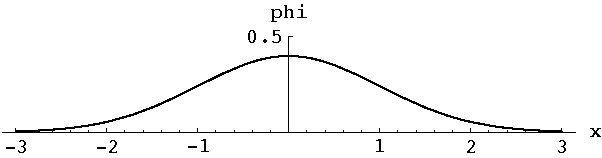
\includegraphics[width=0.8\hsize]{graphics/normphi}
%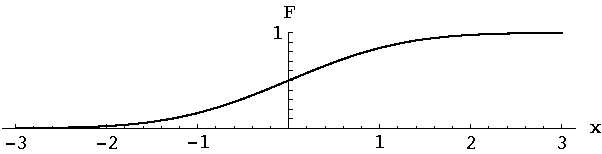
\includegraphics[width=0.8\hsize]{graphics/normF}
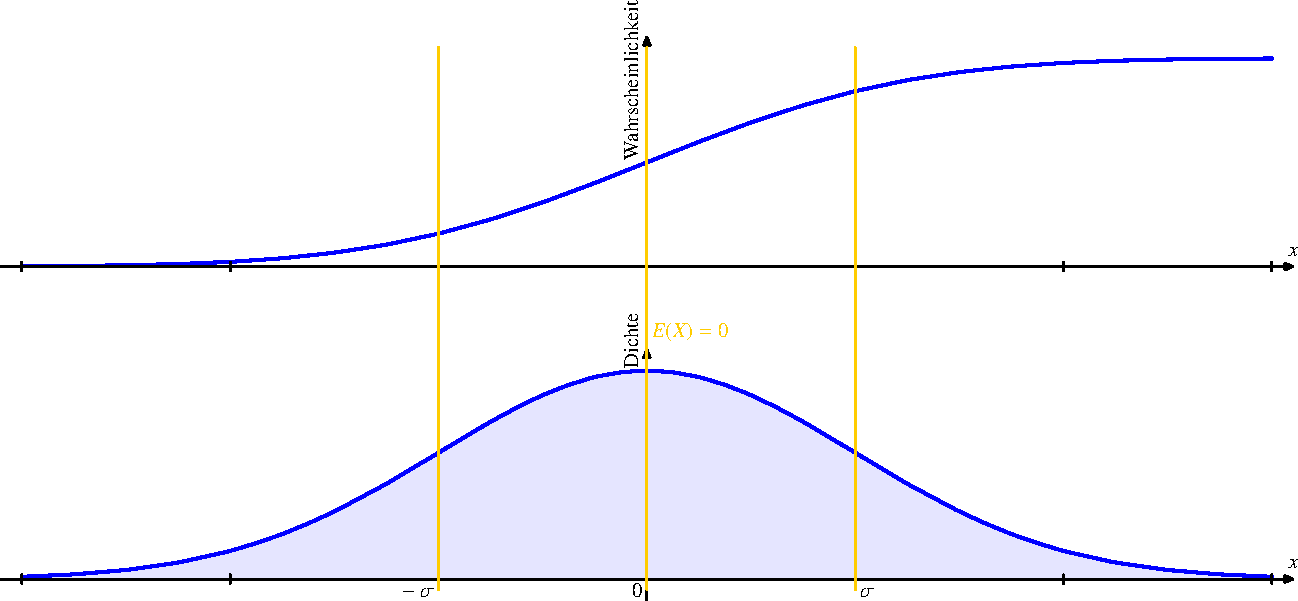
\includegraphics[width=\hsize]{images/verteilungsfunktion-9}
\end{center}
\caption{Dichtefunktion (oben) und Verteilungsfunktion (unten) der Normalverteilung\label{bildnormalverteilung}}
\end{figure}
Die Normalverteilung, auch Gaussverteilung genannt, ist von grosser praktischer
Bedeutung. In sehr vielen Anwendungssituationen darf man davon ausgehen,
dass die beobachteten Zufallsgr"ossen normalverteilt sind. Die Begr"undung
f"ur diesen "uberraschenden Sachverhalt liefert der zentrale Grenzwert-Satz,
welcher im wesentlich besagt, dass eine Zufallsvariable, die als Summe vieler
kleiner, unabh"angiger Zufallseinfl"usse betrachtet werden kann, immer
angen"ahert normalverteilt ist. Wir werden diesen Satz in einem sp"ateren
Abschnitt genauer formulieren.

\subsubsection{Dichtefunktion, Erwartungswert und Varianz}
\index{Wahrscheinlichkeitsdichte!der Normalverteilung}
\index{Normalverteilung!Wahrscheinlichkeitsdichte}
\begin{definition}
Eine Zufallsvariable $X$ heisst normalverteilt mit Erwartungswert $\mu$ und
Varianz $\sigma^2$, wenn sie die
Dichtefunktion
\[
\varphi(x)=\frac1{\sigma\sqrt{2\pi}}e^{-\frac{1}{2}
\left(\frac{x-\mu}{\sigma}\right)^2}
\]
hat.
\end{definition}
\index{Standardnormalverteilung}
\index{Normalverteilung!Standard-}
Die Verteilungsfunktion der Normalverteilung mit Erwartungswert 0
und Varianz 1, der sogenannten Standardnormalverteilung, kann nicht in
geschlossener Form gefunden werden. Man kann sie aber wie folgt
zu berechnen versuchen:
\begin{eqnarray*}
P(X\le x)
&=&\frac1{\sqrt{2\pi}}\int_{-\infty}^xe^{-\frac12\xi^2}\,d\xi\\
&=&\frac12+\frac1{\sqrt{2\pi}}\int_0^xe^{-\frac12\xi^2}\,d\xi\\
&=&\frac12+\frac1{\sqrt{\pi}}\int_0^xe^{-\frac12\xi^2}\,\frac{d\xi}{\sqrt{2}}\\
&=&\frac12+\frac1{\sqrt{\pi}}\int_0^{\frac{x}{\sqrt{2}}}e^{-t^2}\,dt\\
\end{eqnarray*}
Der zweite Term kann mit Hilfe der Fehlerfunktion 
\[
\operatorname{erf}(x)=\frac{2}{\sqrt{\pi}}\int_0^xe^{-t^2}\,dt
\]
umgeformt werden:
\[
P(X\le x)=\frac12\biggl(1+\operatorname{erf}\biggl(\frac{x}{\sqrt{2}}\biggr)\biggr).
\]
\index{Fehlerfunktion}
\index{Verteilungsfunktion!Normalverteilung}
Die Fehlerfunktion ist eine ungerade Funktion mit Wertebereich $(-1,1)$,
sie ist in vielen Softwaresystemen als Bibliotheksfunktion verf"ugbar, in
der C-Bibliothek steht zum Beispiel neben $\operatorname{erf}(x)$ auch
$1-\operatorname{erf}(x)$ zur Verf"ugung.
Da $\lim_{x\to\infty}\operatorname{erf}(x)=1$ k"onnten Werte von
$1-\operatorname{erf}(x)$ f"ur grosse Werte von $x$ nur mit grossen Fehlern 
berechnet werden, die komplement"are Fehlerfunktion l"ost dieses Problem.

Der Vollst"andigkeit halber rechnen wir nach, ob die durch $\varphi$
definierte Verteilung tats"achlich die behaupteten Eigenschaften hat.
Zun"achst hat man die allgemeine Formel:
\begin{eqnarray*}
\int_{-\infty}^{\infty}f(x)\varphi(x)\,dx
&=&\frac1{\sigma\sqrt{2\pi}}\int_{-\infty}^{\infty}f(x)e^{-\frac{1}{2}\left(\frac{x-\mu}{\sigma}\right)^2}\,dx\\
&=&\frac1{\sqrt{2\pi}}\int_{-\infty}^{\infty}f(\sigma\xi+\mu)e^{-\frac{\xi^2}2}\,d\xi
\end{eqnarray*}
Daraus kann man jetzt den Erwartungswert bestimmen indem man $f(x)=x$ verwendet:
\begin{eqnarray*}
E(X)
&=&\frac1{\sqrt{2\pi}}\int_{-\infty}^{\infty}(\sigma\xi+\mu)e^{-\frac{\xi^2}2}\,d\xi\\
&=&\sigma\frac1{\sqrt{2\pi}}\int_{-\infty}^{\infty}\xi e^{-\frac{\xi^2}2}\,d\xi+
\mu\frac1{\sqrt{2\pi}}\int_{-\infty}^{\infty}e^{-\frac{\xi^2}2}\,d\xi\\
\end{eqnarray*}
F"ur das erste Integral benutzt man
\[
\frac{d}{d\xi}e^{-\frac{\xi^2}{2}}=-\xi e^{-\frac{\xi^2}{2}}
\]
woraus folgt
\[
\frac1{\sqrt{2\pi}}\int_{-\infty}^{\infty}\xi e^{-\frac{\xi^2}2}\,d\xi
=
-\frac1{\sqrt{2\pi}}\left[
 e^{-\frac{\xi^2}2}
\right]_{-\infty}^{\infty}=0
\]
Um das zweite Integral benutzt man wir den Trick, dass wir dessen
Quadrat bestimmen:
\begin{eqnarray*}
\biggl(\frac{1}{\sqrt{2\pi}}\int_{-\infty}^{\infty}e^{-\frac{x^2}2}\,dx\biggr)^2
&=&
\frac1{\sqrt{2\pi}}\int_{-\infty}^{\infty} e^{-\frac{\xi^2}2}\,d\xi\cdot
\frac1{\sqrt{2\pi}}\int_{-\infty}^{\infty} e^{-\frac{\eta^2}2}\,d\eta\\
&=&
\frac1{2\pi}\int_{-\infty}^{\infty}\int_{-\infty}^{\infty}
e^{-\frac{\xi^2+\eta^2}2}
\,d\xi\,d\eta\\
&=&
\frac1{2\pi}\int_{0}^{\infty}\int_{0}^{2\pi}re^{-\frac{r^2}2}\,d\varphi\,dr\\
&=&\int_0^{\infty}re^{-\frac{r^2}2}\,dr
=\bigl[-e^{-\frac{r^2}2}\bigr]_0^{\infty}
=1\\
\end{eqnarray*}
Dabei haben wir in der dritten Zeile auf Polarkoordinaten gewechselt.
Somit ist $E(X)=\mu$.

\index{Erwartungswert!Normalverteilung}
\index{Normalverteilung!Erwartungswert}
\index{Varianz!Normalverteilung}
\index{Normalverteilung!Varianz}
F"ur die Varianz von $(x-\mu)$ k"onnen wir annehmen, dass $\mu=0$, dann
gen"ugt es, $E(X^2)$ zu berechnen:
\begin{eqnarray*}
E(X^2)
&=&\frac1{\sqrt{2\pi}}\int_{-\infty}^{\infty}(\sigma\xi)^2e^{-\frac{\xi^2}2}\,d\xi\\
&=&\sigma^2\frac{1}{\sqrt{2\pi}}\int_{-\infty}^{\infty}\xi^2e^{-\frac{\xi^2}2}\,d\xi
\end{eqnarray*}
Das Integral kann durch partielle Integration mit den Faktoren
$\xi$ und $\xi e^{-\frac{\xi^2}2}$ vereinfacht werden:
\begin{eqnarray*}
E(X^2)
&=&\sigma^2\frac{1}{\sqrt{2\pi}}\int_{-\infty}^{\infty}\xi^2e^{-\frac{\xi^2}2}\,d\xi\\
&=&\sigma^2\frac{1}{\sqrt{2\pi}}\biggl(
\biggl[\xi e^{-\frac{\xi^2}2}\biggr]_{-\infty}^{\infty}
+
\int_{-\infty}^{\infty}e^{-\frac{\xi^2}2}\,d\xi
\biggr)\\
&=&\sigma^2\frac{1}{\sqrt{2\pi}}
\int_{-\infty}^{\infty}e^{-\frac{\xi^2}2}\,d\xi\\
&=&\sigma^2
\end{eqnarray*}
Also ist $\operatorname{var}(X)=\sigma$.

Integrale von Ausdr"ucken der Form
$e^{-\frac12(ax^2+bx+c)}$
kommen beim Rechnen mit der Normalverteilung immer wieder vor, deshalb
stellen wir das Resultat in Form eines Hilfssatzes bereit:
\begin{hilfssatz}
\label{exp-quadr}
Ist $a>0$, dann gilt
\[
\frac1{\sqrt{2\pi}}\int_{-\infty}^{\infty}\exp\left(-\frac12(ax^2+bx+c)\right)\,dx
=
\frac1{\sqrt{a}}\exp\left(-\frac12\left(c-\frac{b^2}{4a}\right)\right).
\]
\end{hilfssatz}
\begin{proof}[Beweis]
Durch quadratisches Erg"anzen kann man den Ausdruck $ax^2+bx+c$ umschreiben in
\[
ax^2+bx+c=a\left(x-\frac{b}{2a}\right)^2+c-\frac{b^2}{4a}.
\]
Damit l"asst sich das Integral wie folgt vereinfachen:
\begin{eqnarray*}
&&\frac1{\sqrt{2\pi}}\int_{-\infty}^{\infty}\exp\biggl(-\frac12\biggl(
a\biggl(x-\frac{b}{2a}\biggr)^2+c-\frac{b^2}{4a}
\biggr)\biggr)\,dx\\
&=&\frac1{\sqrt{2\pi}}
\exp\biggl(-\frac12\biggl(
c-\frac{b^2}{4a}
\biggr)\biggr)
\int_{-\infty}^{\infty}
\exp\biggl(-\frac12\biggl(
a\biggl(x-\frac{b}{2a}\biggr)^2
\biggr)\biggr)
\,dx\\
&=&
\exp\biggl(-\frac12\biggl(
c-\frac{b^2}{4a}
\biggr)\biggr)
\frac1{\sqrt{2\pi}}
\int_{-\infty}^{\infty}
\exp\left(-\frac12
a\xi^2
\right)
\,d\xi\\
&=&
\exp\biggl(-\frac12\biggl(
c-\frac{b^2}{4a}
\biggr)\biggr)
\frac1{\sqrt{2\pi}}
\int_{-\infty}^{\infty}
\exp\left(-\frac12
\eta^2
\right)
\,\frac{d\eta}{\sqrt{a}}\\
&=&
\frac{1}{\sqrt{a}}
\exp\biggl(-\frac12\biggl(
c-\frac{b^2}{4a}
\biggr)\biggr)
\end{eqnarray*}
Wobei wir in der dritten Zeile die Substitution $\xi=x-\frac{b}{2a}$
und in der vierten die Substitution
$\eta=\sqrt{a}\xi$
verwendet haben.
\end{proof}

\subsubsection{Summe normalverteilter Zufallsvariablen}
\index{Summe normalverteilter Zufallsvariablen}
\index{Faltung der Normalverteilung}

Eine besonders wichtige Eigenschaft der Normalverteilung ist, dass die
Summe zweier unabh"angiger normalverteilter Zufallsgr"ossen wieder normalverteilt
ist.
\begin{satz}
Sind $X_1$ und $X_2$ normalverteilte Zufallsgr"ossen mit Mittelwert $\mu_1$
resp.~$\mu_2$ und Varianz $\sigma_1$ resp.~$\sigma_2$, dann ist
$X_1+X_2$ ebenfalls normalverteilt mit Mittelwert $\mu_1+\mu_2$ und
Varianz $\sigma^2=\sigma_1^2+\sigma_2^2$.
\end{satz}
\begin{proof}[Beweis]
Aus der Linearit"at des Erwartungswertes ist klar, dass der Mittelwert
$\mu=\mu_1+\mu_2$ sein muss.
Auch wissen wir bereits aus Satz \ref{rechenregeln-varianz}, dass
die Varianz der Summe $X_1+X_2$ die angegebene Form hat. Es ist also nur
noch nachzupr"ufen, dass die Dichtefunktion wieder die eine Normalverteilung
ist.

Zun"achst haben offensichtlich $X_1$ und $X_1-\mu_1$ Dichtefunktionen,
die sich nur durch eine Translation um $\mu_1$  unterscheiden, ebenso
$X_2$ und $X_1+X_2$. Es gen"ugt also, den Fall $\mu_1=\mu_2=0$
zu untersuchen.

Wir berechnen die Dichtefunktion der Verteilung der Summe $X=X_1+X_2$
mit Hilfe der Faltung. 
Dazu muss das Integral 
\begin{eqnarray*}
\varphi_1*\varphi_2(z)
&=&
\int_{-\infty}^{\infty}\varphi_1(t)\varphi_2(z-t)\,dt\\
&=&
\int_{-\infty}^{\infty}
\frac1{\sigma_1\sqrt{2\pi}}e^{-\frac12\left(\frac{t}{\sigma_1}\right)^2}
\frac1{\sigma_2\sqrt{2\pi}}e^{-\frac12\left(\frac{z-t}{\sigma_2}\right)^2}
\,dt\\
&=&
\frac1{\sigma_1\sqrt{2\pi}}
\frac1{\sigma_2\sqrt{2\pi}}
\int_{-\infty}^{\infty}
e^{-\frac12\left(\frac{t}{\sigma_1}\right)^2}
e^{-\frac12\left(\frac{z-t}{\sigma_2}\right)^2}
\,dt\\
&=&
\frac1{\sigma_1\sqrt{2\pi}}
\frac1{\sigma_2\sqrt{2\pi}}
\int_{-\infty}^{\infty}
\exp\biggl(-\frac12\biggl[\biggl(\frac{t}{\sigma_1}\biggr)^2
+\left(\frac{z-t}{\sigma_2}\right)^2\biggr]\biggr)
\,dt
\end{eqnarray*}
ausgewertet werden. Im Exponenten in der eckigen Klammer steht der Ausdruck
\[
\biggl(\frac{t}{\sigma_1}\biggr)^2 +\left(\frac{z-t}{\sigma_2}\right)^2,
\]
den wir durch Ausmultiplizieren in die Form
\[
\biggl(\frac1{\sigma_1^2}+\frac1{\sigma_2^2}\biggr)t^2
-\frac{2z}{\sigma_2^2}t+\frac{z^2}{\sigma_2^2}
\]
bringen k"onnen. Das ist genau die Form, f"ur das im Hilfssatz \ref{exp-quadr}
ein Resultat bereitgestellt wurde, wobei jetzt folgende Werte f"ur $a$, $b$ und $c$
zu verwenden sind:
\[
a=\left(\frac1{\sigma_1^2}+\frac1{\sigma_2^2}\right)
=\frac{\sigma_1^2+\sigma_2^2}{\sigma_1^2\sigma_2^2},\qquad
b=\frac{2z}{\sigma_2^2},\qquad
c=\frac{z^2}{\sigma_2^2}
\]
Setzt man diese Werte in das Resultat von Hilfssatz \ref{exp-quadr} ein,
ergibt sich
\begin{eqnarray*}
\varphi_1*\varphi_2(z)
&=&
\frac1{\sigma_1\sqrt{2\pi}}
\frac1{\sigma_2\sqrt{2\pi}}
\int_{-\infty}^{\infty}
\exp\biggl(-\frac12\biggl[\biggl(\frac{t}{\sigma_1}\biggr)^2
+\left(\frac{z-t}{\sigma_2}\right)^2\biggr]\biggr)
\,dt\\
&=&
\frac1{\sqrt{\sigma_1^2+\sigma_2^2}\sqrt{2\pi}}
\exp\biggl(-\frac12\biggl[c-\frac{b^2}{4a} \biggr]\biggr)
\end{eqnarray*}
Der Ausdruck in der eckigen Klammer wird zu
\begin{eqnarray*}
c-\frac{b^2}{4a}
&=&
\frac{z^2}{\sigma_2^2}
-
\frac{4z^2}{\sigma_2^4}
\frac{\sigma_1^2\sigma_2^2}{\sigma_1^2+\sigma_2^2}
\frac14\\
&=&
\frac{z^2}{\sigma_2^2}
-
\frac{z^2}{\sigma_2^2}
\frac{\sigma_1^2}{\sigma_1^2+\sigma_2^2}
=
\frac{z^2}{\sigma_2^2}
\left(
1-\frac{\sigma_1^2}{\sigma_1^2+\sigma_2^2}
\right)\\
&=&
\frac{z^2}{\sigma_2^2}
\frac{\sigma_2^2}{\sigma_1^2+\sigma_2^2}
=
\frac{z^2}
{\sigma_1^2+\sigma_2^2}
\end{eqnarray*}
Woraus sich f"ur das Faltungsprodukt
\begin{eqnarray*}
\varphi_1*\varphi_2(z)
&=&
\frac1{\sqrt{\sigma_1^2+\sigma_2^2}\sqrt{2\pi}}
\exp\biggl(-\frac12\frac{z^2}{\sigma_1^2+\sigma_2^2}\biggr)
\end{eqnarray*}
ergibt, was genau die Wahrscheinlichkeitsdichte der Normalverteilung
mit Varianz $\sqrt{\sigma_1^2+\sigma_2^2}$ darstellt.
\end{proof}

\subsubsection{Wahrscheinlichkeit grosser Abweichungen}
\begin{figure}
\begin{center}
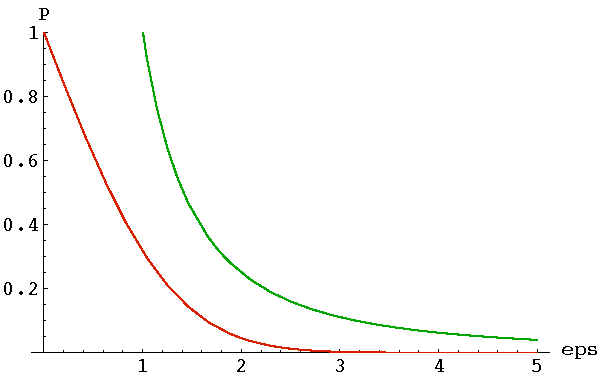
\includegraphics[width=0.8\hsize]{graphics/abwnorm}
\end{center}
\caption{Vergleich der Wahrscheinlichkeit f"ur eine grosse Abweichung
f"ur die Normalverteilung (rot) und die Schranke von Tschebyscheff (gr"un)
\label{abweichung-normalverteilung}}
\end{figure}

Auch f"ur die Normalverteilung wollen wir die Wahrscheinlichkeit
f"ur grosse Abweichungen berechnen. Es gilt wieder
\[
P(|X-\mu|>\varepsilon)
=1-\int_{-\varepsilon}^{\varepsilon}e^{-\frac{x^2}{2\sigma^2}}\,dx
=
1-{\textstyle\frac12}(\operatorname{erf}({\textstyle\frac{\varepsilon}{\sigma\sqrt{2}}})-\operatorname{erf}({\textstyle-\frac{\varepsilon}{\sigma\sqrt{2}}}))
=
1-\operatorname{erf}({\textstyle\frac{\varepsilon}{\sigma\sqrt{2}}})
\]
Die Abbildung~\ref{abweichung-normalverteilung} zeigt die Wahrscheinlichkeit
f"ur eine grosse Abweichung vom Mittelwert ein Einheiten
von $\sqrt{\operatorname{var}(X)}$. Noch deutlicher als bei der
Exponentialverteilung zeigt sich, dass die zus"atzliche Information
"uber die Verteilung die Wahrscheinlichkeit f"ur eine grosse
Abweichung deutlich besser absch"atzen l"asst.

\subsubsection{Der zentrale Grenzwertsatz}
\label{zentraler-grenzwertsatz}
\index{Zentraler Grenzwertsatz}
\index{Grenzwertsatz, zentraler}
\index{Normalapproximation}
In vielen Anwendunge sieht man die Zufallsprozesse nicht einzeln, sondern
man sieht eine grosse Zahl von Zufallsprozessen, die zusammenwirken.
So entsteht der Druck, den ein Gas auf die Wand seines Beh"alters aus"ubt,
durch die grosse Zahl von unabh"angigen St"ossen der einzelnen Gasteilchen
auf die Wand. Das Rauschen in einer elektrischen Schaltung setzt sich
zusammen aus vielen einzelnen Beitr"agen, die zum Beispiel in einzelnen
Bauteilen entstehen, und dort durch das Zusammenspiel der zuf"alligen
thermischen Bewegung der Atome hervorgerufen werden.
Dieses Zusammenspiel von vielen kleinen Zufallsfaktoren soll in diesem
Abschnitt modelliert werden.

Wir gehen dazu von einer Folge von unabh"angigen Zufallsvariablen
\[
X_1,X_2,X_3,\dots
\]
aus, die alle Erwartungswert $0$ und Varianz $1$ haben, also
\[
E(X_i)=0\quad\wedge\quad\operatorname{var}(X_i)=1\qquad\forall i.
\]
Aus diesen Zufallsvariablen werden nun neue Zufallsvariablen
\[
S_n=\frac{X_1+\dots+X_n}{\sqrt{n}}
\]
gebildet, welche wiederum Erwartungswert $0$ und Varianz $1$ haben,
weil
\[
\operatorname{var}(S_n)=\operatorname{var}\bigl(\frac1{\sqrt{n}}(X_1+\dots+X_n)\big)
=\frac1n\operatorname{var}(X_1+\dots+X_n)
\]
ist. Die Summe $S_n$ beschreibt das Zusammenwirken der ersten $n$
Zufallsvariablen $X_i$. Die einzelnen Faktoren k"onnen "ublicherweise
nicht beobachtet werden, nur $S_n$ ist der Messung zug"anglich.

In der Physik lernt man, dass man die st"andige, zufallsbestimmte
Bewegung der Atome in einem Gas oder K"orper nicht im Detail
zu verstehen braucht, und trotzdem eine n"utzliche W"armelehre
aufstellen kann. Daher sollte es m"oglich sein, "uber die Verteilung
$S_n$ mindestens f"ur sehr grosse $n$ etwas auszusagen, selbst
wenn "uber die einzelnen Beitr"age $X_i$ nur sehr wenig bekannt ist.
\begin{figure}
\begin{center}
%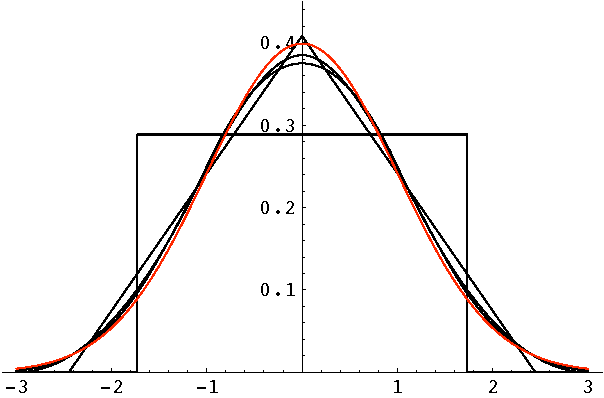
\includegraphics[width=0.8\hsize]{graphics/zgws}
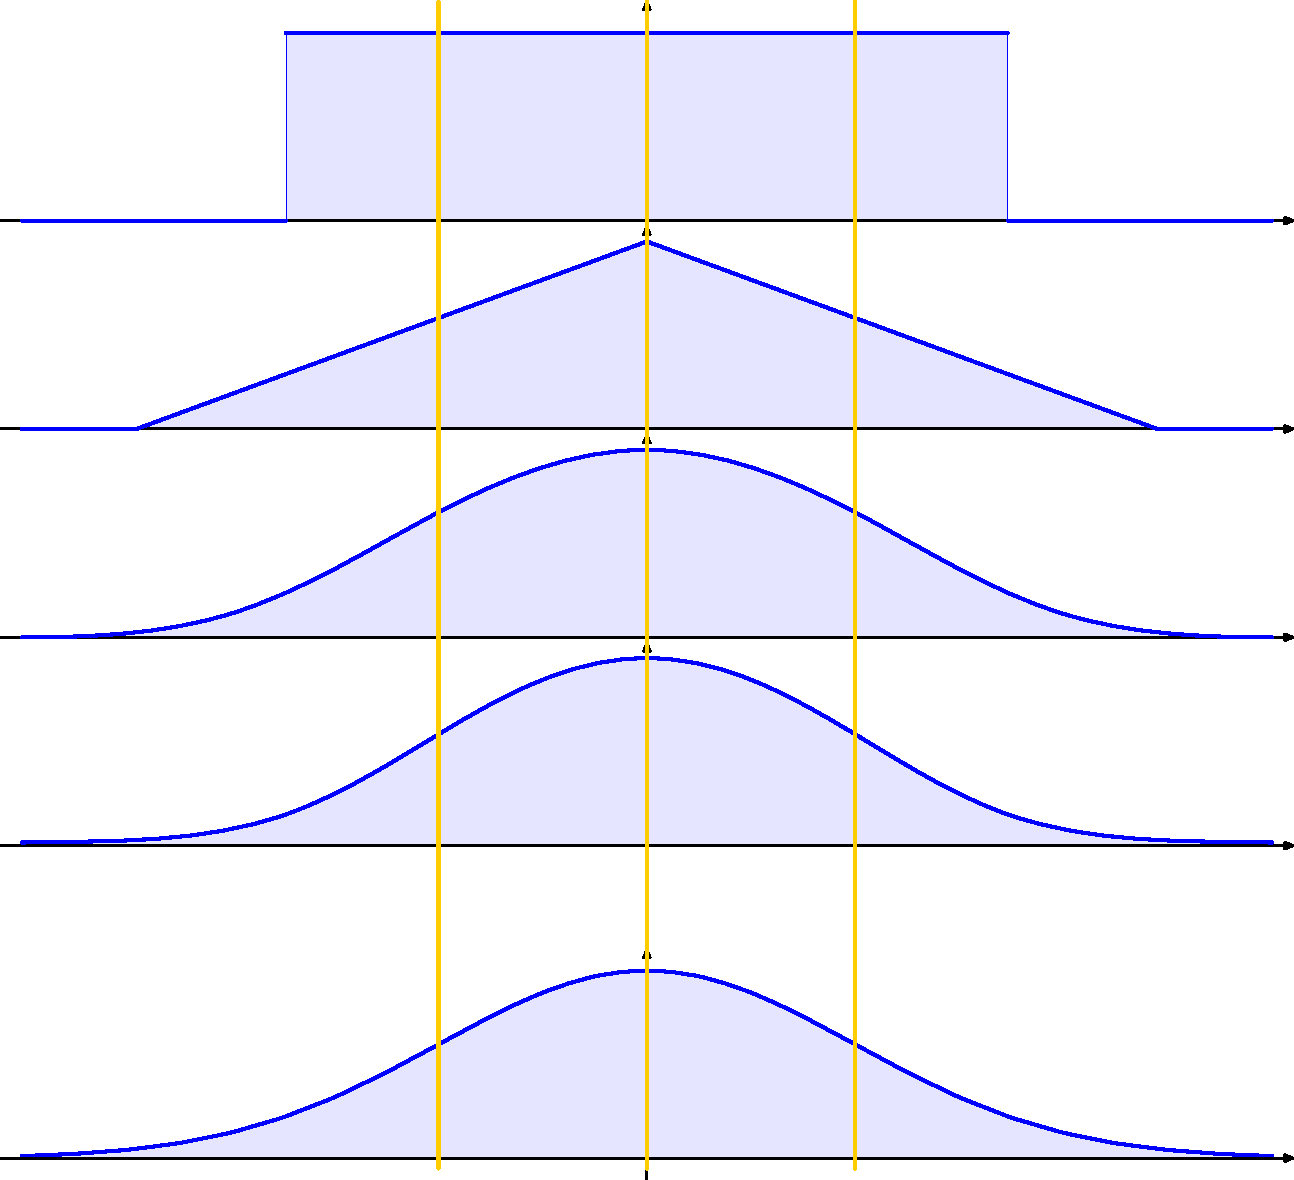
\includegraphics[width=\hsize]{images/verteilungsfunktion-10}
\end{center}
\caption{Zum zentralen Grenzwertsatz: die Wahrscheinlichkeitsdichte
der standardisierten Summe von bis zu vier 
gleichverteilten Zufallsvariablen (oben)
konvergiert gegen die Standardnormalverteilung (unten).\label{zgws}}
\end{figure}

Der zentrale Grenzwertsatz besagt nun, dass die Verteilungsfunktionen
von $S_n$ gegen die Verteilungsfunktion einer Normalverteilung
konvergieren\footnote{Wie genau diese Konvergenz gemeint ist, wird
im Laufe der Berechnung klar werden.}. In den folgenden Abschnitten
versuchen wir, die Verteilungsfunktion von $S_n$ und insbesondere
ihren Grenzwert zu berechnen. Die Abbildung \ref{zgws} illustriert
dies: dort wird die Wahrscheinlichkeitsdichte der standardisierten
Summe von bis zu vier im
Intervall $[-\sqrt{3},\sqrt{3}]$ gleichverteilte Zufallsvariablen dargestellt,
und mit der Standardnormallverteilung verglichen.

Wir betrachten als technisches Hilfsmittel f"ur die Berechnung
die folgende Funktion:
\index{momenterzeugende Funktion}
\begin{definition} Ist $X$ eine Zufallsvariable, dann heisst die Funktion
\marginpar{\raggedright\tiny momenterzeugende Funktion}
\[
M_X(t)=t\mapsto E(e^{tX})=\sum_{k=0}^n\frac{t^k}{k!}E(X^k).
\]
die momenterzeugende Funktion von $X$
\end{definition}
Wir nehmen im folgenden
an, dass diese Funktion existiert\footnote{F"ur alle in diesem Kapitel
untersuchten Verteilungen trifft dies zu, es gibt aber auch Verteilungen,
f"ur die die momenterzeugende Funktion nicht existiert, f"ur die der
zentrale Grenzwertsatz aber trotzdem gilt.}. F"ur die momenterzeugende
\marginpar{\raggedright\tiny Rechenregeln f"ur die momenterzeugende Funktion}
Funktion gilt die folgende Rechenregeln
\begin{eqnarray*}
M_{X+Y}(t)&=&M_X(t)M_Y(t)\\
M_{\lambda X}(t)&=&M_X(\lambda t)
\end{eqnarray*}

Wenn $\varphi$ die Dichtefunktion zur Zufallsvariable $X$ ist, dann
kann die momenterzeugende Funktion wie folgt berechnet werden:
\[
M_X(t)=E(e^{tX})=\int_{-\infty}^\infty e^{tx}\varphi(x)\,dx,
\]
die momenterzeugende Funktion ist also nichts anderes als eine
zweiseitige Laplacetransformierte von $\varphi$:
\[
M_X(t)={\cal L}\varphi(-t),
\]
insbesondere l"asst sich in vielen F"allen aus der Laplacetransformierten
die urspr"ungliche Funktion wieder bestimmen.
Der Plan ist daher der folgende:
\begin{enumerate}
\item Bestimme einen N"aherungsausdruck f"ur $M_{X_i}(t)$.
\item Bestimme einen N"aherungsausdruck f"ur $M_{S_n}(t)$.
\item Berechne den Grenzwert von $M_{S_n}(t)$ f"ur $n\to\infty$.
\item Finde eine Verteilung, die die gleiche Laplacetransformation
hat.
\end{enumerate}

{\parindent0pt\bf 1.~Schritt: N"aherung f"ur $M_{X_i}(t)$.} 
\index{Taylorreihe}
Aus der Taylorentwicklung von $e^{tX}$ folgt
\[
M_{X_i}(t)=1+E(X)t+\operatorname{var}(X)\frac{t^2}{2!}+R_i(t)t^2
=1+\frac{t^2}{2!}+R_i(t)t^2
\]
Dabei ist das Restglied $R_i(t)$ so beschaffen, dass
$R_i(t)\to 0$ wenn $t\to 0$.

\medskip
{\parindent0pt\bf 2.~Schritt: Berechnung von $M_{S_n}(t)$.}
Aus den beiden Rechenregeln f"ur die momenterzeugende Funktion folgt
jetzt zun"achst f"ur die Summe der Zufallsvariablen
\[
M_{X_1+\dots+X_n}(t)=M_{X_1}(t)\dots M_{X_n}(t),
\]
und anschliessen f"ur das Produkt mit $\frac1{\sqrt{n}}$
\[
M_{S_n}(t)=M_{X_1}(t/\sqrt{n})\dots M_{X_n}(t/\sqrt{n}).
\]
Durch Einsetzen der N"aherung aus dem ersten Schritt ergibt sich
\[
M_{S_n}(t)
=\prod_{i=1}^n\biggl(1+\frac{t^2}{2n}+R_i\biggl(\frac{t}{\sqrt{n}}\biggl)\frac{t^2}{n}\biggr)
=\biggl(1+\frac{t^2}{2n}+Q_n\biggl(\frac{t}{\sqrt{n}}\biggr)\frac{t^2}{n}\biggr)^n,
\]
wobei $Q_n(t)$ eine neue Funktion ist. Diese kann durch
\[
Q_n(t/\sqrt{n})=\root{n}\of{M_{S_n}(t)}-1-\frac{t^2}{2n}
\]
ermittelt werden, und hat immer noch die Eigenschaft,
$\lim_{t\to0}Q_n(t)=0$. Im einfachsten Fall, wenn die Zufallsvariablen
identisch verteilt sind, sind alle Funktionen $R_i$ gleich, und damit
auch alle $Q_n$.

\medskip
{\parindent0pt\bf 3.~Schritt: Grenzwert f"ur $n\to\infty$.}
F"ur den Grenz"ubergang $n\to\infty$ beachten wir nun, schreiben wir
$M_{S_n}(t)$ mit Hilfe von
$x_n=\frac{t^2}2+Q_n(t)$
um als
\[
M_{S_n}(t)=\biggl(1+\frac{x_n}n\biggr)^n
\]
Nun ist bereits aus der Analysis bekannt, dass
\[
\lim_{n\to\infty}\biggl(1+\frac{x}{n}\biggr)^n=e^x,
\]
es gilt aber auch in verallgemeinerter Form:
\[
\biggl(1+\frac{x_n}{n}\biggr)^n\to e^x\quad\text{falls}\quad x_n\to x.
\]
Da in unserem Fall $x_n\to \frac{t^2}2$ erhalten wir
\[
\lim_{n\to\infty}M_{S_n}(t)=e^{\frac{t^2}{2}}
\]

\medskip
{\parindent0pt\bf 4.~Schritt: Die Grenzverteilung.}
Der gefundene Grenzwert soll die momenterzeugende Funktion einer
Verteilung sein, und wir erwarten, dass sie ebenfalls eine
momenterzeugende Funktion hat. Da die momenterzeugende Funktion
nichts anderes als eine Laplacetransformation ist, k"onnen wir
den Eindeutigkeitssatz f"ur die Laplacetransformation anwenden,
welcher besagt, dass zwei Funktionen, die die gleiche zweiseitige
Laplacetransformierte haben, fast "uberall gleich sein.

Wir rechnen nach, dass $e^{\frac{t^2}2}$ die momenterzeugende Funktion
der Standardnormalverteilung ist. Wir berechnen
dazu die Momente der Normalverteilung $\frac1{\sqrt{2\pi}}e^{-\frac{x^2}2}$
\begin{eqnarray*}
\int_{-\infty}^\infty e^{-\frac{x^2}2}x^{2k+1}\,dx&=&0\\
\int_{-\infty}^\infty e^{-\frac{x^2}2}x^{2k}\,dx
&=&
\biggl[\frac{x^{2k+1}}{2k+1}e^{-\frac{x^2}2}\biggr]_{-\infty}^\infty
+\frac1{(2k+1)}\int_{-\infty}^\infty x^{2k+2}e^{-\frac{x^2}2}\,dx\\
&=&
\frac1{(2k+1)}\int_{-\infty}^\infty x^{2k+2}e^{-\frac{x^2}2}\,dx
\end{eqnarray*}
Insbesondere kann man das $2k+2$-te Moment mit Hilfe einer
Rekursionsformel aus dem $2k$-ten Moment berechnen:
\[
E(X^{2k+2})=(2k+1)E(X^{2k}).
\]
Das $2k$-te Moment ist die Varianz, also $E(X^2)=1$. Damit kann
man die momenterzeugende Funktion von $e^{-\frac{x^2}2}$ aufschreiben:
\begin{eqnarray*}
M(t)
&=&
1+\frac{t^2}{2!} +\frac{t^4}{4!}3 +\frac{t^6}{6!}3\cdot5 +\frac{t^8}{8!}3\cdot5\cdot7+\dots\\
&=&
1+\frac{t^2}{1!\cdot 2^1} +\frac{t^4}{2! \cdot 2^2} +\frac{t^6}{3!\cdot 2^3}
+\frac{t^8}{4!\cdot 2^4}\\
&=&
1+(t^2/2) +\frac{(t^2/2)^2}{2!} +\frac{(t^2/2)^3}{3!}
+\frac{(t^2/2)^4}{4!}\\
&=&e^{\frac{t^2}2}
\end{eqnarray*}
Mit anderen Worten, die momenterzeugende Funktion der Normalverteilung
stimmt "uberein mit der momenterzeugenden Funktion der Grenzverteilung.
Schreiben $\varphi_n$ f"ur die Dichtefunktion f"ur $S_n$ und $F_n$
f"ur die Verteilungsfunktion, dann gilt
nach allgemeinen S"atzen "uber die Laplacetransformation gilt daher
\[
\lim_{n\to\infty}\varphi_n(x)=\frac1{\sqrt{2\pi}}e^{-\frac{x^2}2}
\quad\text{fast "uberall}
\]
und f"ur die Verteilungsfunktion
\[
\lim_{n\to\infty}F_n(x)=\frac1{\sqrt{2\pi}}\int_{-\infty}^xe^{-\frac{t^2}2}\,dt
\]
Insgesamt haben wir damit den folgenden Satz bewiesen
\begin{satz}[Zentraler Grenzwertsatz]
Sind $(X_i)_{1\le i}$ unabh"angige Zufallsvariable mit
Erwartungswert $E(X_i)=0$ und Varianz $\operatorname{var}(X_i)=1$
f"ur alle $i\ge 1$. Dann ist
\[
S_n=\frac1{\sqrt{n}}\sum_{i=1}^nX_i=\frac1{\sqrt{n}}(X_1+\dots+X_n)
\]
eine Folge von Zufallsvariablen, die ebenfalls Erwartungswert $E(S_n)=0$
und Varianz $\operatorname{var}(S_n)=1$ haben. Falls die Zufallsvariablen
$X_i$
f"ur alle $i$ eine momenterzeugende Funktion haben, hat auch $S_n$
f"ur alle $n$ eine momenterzeugende Funktion, ausserdem konvergiert
die Verteilungsfunktion $F_n$ von $S_n$ gegen die Verteilungsfunktion der
Standardnormalverteilung
\[
\lim_{n\to\infty}F_n(x)=\frac1{\sqrt{2\pi}}\int_{-\infty}^xe^{-\frac{t^2}2}\,dt.
\]
Haben die $X_i$ ausserdem eine Wahrscheinlichkeitsdichte,
dann hat auch $S_n$
die Wahrscheinlichkeitsdichte $\varphi_n$, welche fast "uberall gegen die
Wahrscheinlichkeitsdichte der Standardnormalverteilung 
konvergiert:
\[
\lim_{n\to\infty}\varphi_n(x)=\frac1{\sqrt{2\pi}}e^{-\frac{x^2}2}.
\]
\end{satz}

\subsection{$\chi^2$-Verteilung\label{chi2verteilung}}
\index{chi@{$\chi^2$-Verteilung}}
Der zentrale Grenzwertsatz garantiert, dass in vielen praktisch wichtigen
F"allen ann"ahernd normalverteilte Zufallsvariablen vorliegen.
Wenn man nun also weiss, dass die Zufallsvariablen $(X_i)_{1\le i\le n}$
mit Erwartungswert $\mu_i$ und Varianz $\sigma_i^2$ normalverteilt
sind, dann sind die Zufallsvariablen $Y_i=(X_i-\mu_i)/\sigma_i$
standardnormalverteilt. Die meisten $Y_i$ werden also Werte nahe
bei $0$ annehmen, die Summe $\sum_{i=1}^nY_i^2$ wird also im
Allgemeinen klein sein. Grosse Werte der Summe sind sehr unwahrscheinlich.
Treten sie bei einer Beobachtung trotzdem auf, dann ist entweder genau
dieser unwahrscheinliche Fall eingetreten, oder die Annahmen, dass die
$X_i$ normalverteilt waren, ist nicht zutreffend. Somit l"asst sich
aus der Gr"osse ein praktisch n"utzlicher Test konstruieren, ob
eine Normalverteilung vorliegt.

\begin{definition}
Sind $(X_i)_{1\le i\le n}$ standardnormalverteilte Zufallsvariable,
dann ist $\sum_{i=1}^nX_i^2$ eine $\chi^2$-verteilte Zufallsvariable
mit $n$ Freiheitsgraden.
\end{definition}

\begin{satz}\label{chi2}
Die $\chi^2$-Verteilung mit $n$ Freiheitsgraden hat
die Wahrscheinlichkeitsdichte
\[
\gamma_{\frac12,\frac{n}2}(x)=\frac1{\Gamma(\frac{n}2)}\sqrt{\frac1{2^n}x^{n-2}}e^{-\frac12x}\qquad,x\ge 0
\]
Die momenterzeugende Funktion der $\chi^2$-Verteilung ist
\[
\chi_n^2(t)=(1-2t)^{-\frac{n}2}.
\]
\end{satz}

Um diesen Satz zu beweisen, ist es n"utzlich, mehr Information "uber die
Dichtefunktionen zu sammeln. Zun"achst sind die Dichtefunktionen
$\gamma_{\frac12,\frac{n}2}$ Elemente einer viel gr"osseren Familie von
Dichtefunktionen, n"amlich den Gamma-Verteilungen

\subsubsection{Die Gamma-Verteilungen}
\index{gamma@{$\gamma$-Verteilung}}
\begin{definition}
Die Verteilung mit der Dichtefunktion
\[
\gamma_{\alpha,\nu}(x)=\begin{cases}
\displaystyle \frac1{\Gamma(\nu)}\alpha^\nu x^{\nu-1}e^{-\alpha x}&\qquad x>0\\
0&\qquad\text{sonst}
\end{cases}
\]
heist Gamma-Verteilung zum Parameter $(\alpha,\nu)$. Darin ist
\[
\Gamma(t)=\int_0^\infty x^{t-1}e^{-x}\,dx
\]
die Gamma-Funktion.
\end{definition}

Die Gamma-Verteilungen erf"ullen einige interessante Rechenregeln:
\begin{satz} Die Funktionen $\gamma_{\alpha,\nu}$ sind Wahrscheinlichkeitsdichten.
Die Gamma-Verteilungen sind unter Faltung abgeschlossen:
\[
\gamma_{\alpha,\mu}*\gamma_{\alpha,\nu}=\gamma_{\alpha,\mu+\nu}.
\]
Sind $X$ und $Y$ Gamma-verteilte Zufallsvariable, dann ist auch $X+Y$
Gamma-verteilt.
\end{satz}
\begin{proof}[Beweis]
Wir rechnen zun"achst nach, dass $\gamma_{\alpha,\nu}$ tats"achlich
Wahrscheinlichkeitsdichten sind. Dazu ist die Normierung zu pr"ufen:
\begin{eqnarray*}
\int_{-\infty}^\infty \gamma_{\alpha,\nu}(x)\,dx
&=&\int_0^\infty\frac1{\Gamma(\nu)}\alpha^\nu x^{\nu-1}e^{-\alpha x}\,dx\\
&=&\frac{1}{\Gamma(\nu)}\int_0^\infty (\alpha x)^{\nu-1}e^{-\alpha x}
\alpha\,dx\\
&=&\frac1{\Gamma(\nu)}\int_0^\infty \xi^{\nu-1}e^{-\xi}\,d\xi=1
\end{eqnarray*}
Die letzte Gleichung folgt aus der Definition der Gamma-Funktion.

Wir berechnen jetzt das Faltungsprodukt von $\gamma_{\alpha,\mu}$ und
$\gamma_{\alpha,\nu}$, wir wissen bereits, dass das Faltungsprodukt wieder
eine Wahrscheinlichkeitsdichte sein wird. Es gilt
\begin{eqnarray*}
\gamma_{\alpha,\mu}*\gamma_{\alpha,\nu}(x)
&=&\int_{-\infty}^\infty \gamma_{\alpha,\mu}(x-t)\gamma_{\alpha,\nu}(t)\,dt\\
&=&\int_0^x \gamma_{\alpha,\mu}(x-t)\gamma_{\alpha,\nu}(t)\,dt\\
&=&\int_0^x \frac1{\Gamma(\mu)}\alpha^{\mu}(x-t)^{\mu-1}e^{-\alpha (x-t)}
\frac1{\Gamma(\nu)}\alpha^\nu t^{\nu-1}e^{-\alpha t}\,dt\\
&=&\frac{\alpha^{\mu+\nu}e^{-\alpha x}}{\Gamma(\mu)\Gamma(\nu)}\int_0^x
(x-t)^{\mu-1}t^{\nu-1}\,dt\\
&=&\frac{\alpha^{\mu+\nu}e^{-\alpha x}}{\Gamma(\mu)\Gamma(\nu)}x^{\mu+\nu-1}
\int_0^1 (1-\tau)^{\mu-1}\tau^{\nu-1}\,d\tau\\
&=&
\frac1{\Gamma(\mu+\nu)}\alpha^{\mu+\nu}e^{-\alpha x}
x^{\mu+\nu-1}
\cdot
\frac{\Gamma(\mu+\nu)}{\Gamma(\mu)\Gamma(\nu)}
\int_0^1 (1-\tau)^{\mu-1}\tau^{\nu-1}\,d\tau\\
&=&\gamma_{\alpha,\mu+\nu}
\cdot
\frac{\Gamma(\mu+\nu)}{\Gamma(\mu)\Gamma(\nu)}
\int_0^1 (1-\tau)^{\mu-1}\tau^{\nu-1}\,d\tau
\end{eqnarray*}
wobei f"ur die Umformung des Integrals die Substitution $t=x\tau$ verwendet
wurde. Somit ist das Faltungsprodukt bis auf eine konstanten Faktor
wieder eine Gamma-Verteilung, da aber die Gamma-Verteilungen bereits
normiert sind, muss der Faktor eins sein. Als Nebenprodukt erhalten
wir also die Formel
\[
\int_0^1(1-t)^{\mu-1}t^{\nu-1}\,dt=\frac{\Gamma(\mu)\Gamma(\nu)}{\Gamma(\mu+\nu)}.
\]
\end{proof}

\subsubsection{Beweis des Satzes \ref{chi2}}
Die $\chi^2$-Verteilung mit einem Freiheitsgrad ist die Verteilung von
$X^2$, wenn $X$ eine standardnormalverteilte Zufallsvariable ist.
F"ur $x\le 0$ ist die Verteilungsfunktion $F(x)=P(X^2\le x)=0$. 
F"ur $x>0$ gilt
\begin{eqnarray*}
F(x)&=&P(X^2\le x)=P(-\sqrt{x}\le X\le\sqrt{x})\\
&=&\frac1{\sqrt{2\pi}}\int_{-\sqrt{x}}^{\sqrt{x}}e^{-\frac12 \xi^2}\,d\xi\\
&=&\sqrt{\frac{2}{\pi}}\int_0^{\sqrt{x}}e^{-\frac12\xi^2}\,d\xi
\end{eqnarray*}
Mit Hilfe der Substitution $\xi^2=t$ oder $\xi=t^{\frac12}$ k"onnen wir
dies umformen zu
\begin{eqnarray*}
F(x)&=&\frac1{\sqrt{2\pi}}\int_0^xe^{-\frac12t}t^{-\frac12}\,dt\\
&=&\frac1{\sqrt{2\pi}}\int_0^x\gamma_{\frac12,\frac12}(t)
\frac{\Gamma(\frac12)}{{\frac12}^{\frac12}}\,dt
\end{eqnarray*}
Die Ableitung nach $x$ ergibt die Dichtefunktion:
\[
\varphi(x)=\frac1{\sqrt{\pi}}\Gamma({\textstyle\frac12})\gamma_{\frac12,\frac12}(x)
\]
Der Wert der Gamma-Funktion ist
\[
\Gamma({\textstyle\frac12})
=\int_0^\infty x^{-\frac12}e^{-x}\,dx
\]
kann mit der Substitution $x=\xi^2$ berechnet werden,
\[
\Gamma({\textstyle\frac12})=\int_0^\infty \xi^{-1}e^{-\xi^2}2\xi\,d\xi
=\int_0^{\infty}e^{-\xi^2}\,d\xi
\]
Das Integral auf der echten Seite ist bis auf einen Normierungsfaktor
das Integral "uber die Dichte einer Normalverteilung, also
\[
\Gamma({\textstyle\frac12})=\sqrt{\pi},
\]
woraus sich ablesen l"asst, dass die Wahrscheinlichkeitsdichte 
von $X^2$ tats"achlich $\gamma_{\frac12,\frac12}$ ist.

Nun kann man vollst"andige Induktion zusammen mit der Faltungseigenschaft
verwenden. F"ur $n=1$ ist bereits bekannt, dass die Wahrscheinlichkeitsdichte
f"ur $n$ Summanden $X_i^2$ $\gamma_{\frac12,\frac{n}2}$ ist. Nehmen wir an,
dass f"ur $n-1$ Summanden die Wahrscheinlichkeitsdichte
$\gamma_{\frac12,\frac{n-1}2}$
ist, dann erhalten wir f"ur $n$ Summanden mit der Faltungseigenschaft
\[
\gamma_{\frac12,\frac12}*\gamma_{\frac12,\frac{n-1}2}=\gamma_{\frac12,\frac{n}2}.
\]

Es bleibt, die momenterzeugende Funktion von $\chi_n^2$ zu berechnen.
Wegen
\[
M_{\chi_{n-1}^2}(t)M_{\chi_1^2}(t)=M_{\chi_n^2}(t)
\]
gen"ugt es, eine Formel f"ur $M_{\chi_1^2}(t)$ zu finden. Die Dichte
der $\chi_1^2$-Verteilung ist
\[
\frac1{\sqrt{2\pi}}e^{-\frac{x}2}x^{-\frac12}.
\]
Nach Definition der momenterzeugenden Funktion ist
\begin{eqnarray*}
M_{\chi_1^2}(t)
&=&\frac1{\sqrt{2\pi}}\int_0^\infty e^{xt}e^{-\frac{x}2}x^{-\frac12}\,dx\\
&=&\frac1{\sqrt{2\pi}}\int_0^\infty x^{-\frac12}e^{x(t-\frac12)}\,dx\\
&=&\frac1{\sqrt{2\pi}}\int_0^\infty x^{-\frac12}e^{-\alpha x}\,dx\\
&=&\frac1{\sqrt{2\pi}}\frac1{\sqrt{\alpha}}\int_0^\infty\xi^{-\frac12}e^{-\xi}\,d\xi\\
&=&\frac1{\sqrt{2\pi}}\frac1{\alpha}\Gamma(\frac12)=\frac1{2\alpha}\\
&=&\frac1{\sqrt{1-2t}}=(1-2t)^{-\frac12},
\end{eqnarray*}
wobei wir die Subsitutionen $-\alpha=t-\frac12$ und $\alpha x=\xi$
verwendet haben. Somit ist
\[
M_{\chi_1^2}(t)=(1-2t)^{-\frac12},
\]
also auch
\[
M_{\chi_n^2}(t)=(1-2t)^{-\frac{n}2}.
\]
Damit der Satz \ref{chi2} vollst"andig bewiesen ist.

\subsubsection{Normalverteilungstest}
\index{Normalverteilungstest}
Die Zufallsvariablen $X_i$ waren unabh"angig und standardnormalverteilt
vorausgesetzt worden.
Die Gr"osse $\sum_{i=1}^nX_i^2$ liefert einen Test daf"ur, ob die Gr"ossen
$X_i$ tats"achlich standardnormalverteilt sind. Ist zum Beispiel der
Erwartungswert der $X_i$ nicht $0$, dann wird $\sum_{i=1}^nX_i^2$
deutlich gr"osser. Die Hypothese, dass die $X_i$ standardnormalverteilt
sind, kann also verworfen werden, wenn $\sum_{i=1}^nX_i^2$ eine gewisse
Schranke $M$ "uberschreitet. Die Wahrscheinlichkeit, dass die Hypothese
verworfen wird, obwohl sie eigentlich zutrifft, ist
\[
P\biggl(\sum_{i=1}^nX_i^2>M\biggr).
\]
Will man die Wahrscheinlichkeit eines solchen Irrtums klein halten, muss
$M$ entsprechend gross gew"ahlt werden. Wie gross definiert die
$\chi^2$-Verteilung. Soll die Fehlerwahrscheinlichkeit $p$ sein,
dann muss $M$ so gew"ahlt werden, dass 
\[
P\biggl(\sum_{i=1}^nX_i^2>M\biggr)=\int_M^\infty \gamma_{\frac12,\frac{n}2}(t)\,dt = p.
\]
Die Schranke $M$ ist f"ur verschiedene Werte von $p$ in Abh"angigkeit
von der Anzahl Freiheitsgrade tabelliert, oder kann mit dem Computer
berechnet werden.
Zu diesem Zweck ist zum Beispiel in der GNU Scientific
Library die Funktion \verb+gsl_cdf_chisq_Pinv(double p, double nu)+
vorhanden, der Parameter \verb+p+ ist die Wahrscheinlichkeit eines
Fehlers, {\tt nu} ist die Zahl der Freiheitsgrade.

\subsection{Potenzgesetze} \label{potenzgesetze}
\begin{table}
\renewcommand{\arraystretch}{2}
\begin{center}
\begin{tabular}{|l|l|}
\hline
Name&Potenzverteilung, Pareto-Verteilung\\
\hline
Dichtefunktion&
\begin{minipage}{3.7in}
\vskip5pt
$\displaystyle
\begin{cases}
\frac{\alpha-1}{x_{\text{min}}}^{1-\alpha}x^{-\alpha}&\qquad x>x_{\text{min}}\\
0&\qquad\text{sonst}
\end{cases}
$
\end{minipage}
\\[15pt]
Verteilungsfunktion&
\begin{minipage}{3.7in}
\vskip3pt
$\displaystyle
\begin{cases}
1-\biggl(\frac{x}{x_{\text{min}}}\biggr)^{1-\alpha}&\qquad x>x_{\text{min}}\\
0&\qquad\text{sonst}
\end{cases} $
\end{minipage}
\\
Erwartungswert&$\displaystyle\frac{\alpha-1}{\alpha-2}x_{\text{min}}$,
undefiniert f"ur $\alpha\ge 2$\\
Varianz&$\displaystyle
\biggl(
\frac{\alpha-1}{\alpha -3}-\biggl(\frac{\alpha-1}{\alpha-2}\biggr)^2
\biggr)x_{\text{min}}^2$, undefiniert f"ur $\alpha \ge 3$\\
$P(|X-E(X)|>\varepsilon)$&$\displaystyle $ \\
Median&$2^{\frac1{\alpha-1}}x_{\text{min}}$\\
\hline
Anwendungen&\begin{minipage}{3.7in}%
\vskip5pt
\strut
$\bullet$ H"aufkeitsverteilung f"ur skaleninvariante Prozesse\\
$\bullet$ Einkommensverteilung\\
$\bullet$ Gr"osse und H"aufigkeit von Mondkratern\\
$\bullet$ Verkaufszahlen von B"uchern\\
$\bullet$ Einwohnerzahlen von St"adten
\strut
\end{minipage}\\[28pt]
\hline
\end{tabular}
\end{center}
\caption{Datenblatt der Potenzverteilung\label{datenblatt:potenzverteilung}}
\end{table}
Die Normalverteilung beschreibt physikalische Gr"ossen sehr erfolgreich,
die vor allem in einer bestimmten Gr"osse vorkommen. Menschen sind zum
Beispiel im Durchschnitt etwa 1.80m gross, Abweichungen kommen vor, sind
aber sehr selten, 5m grosse Menschen gibt es nicht.

Andererseits gibt es auch Gr"ossen, die einen weiten Bereich von m"oglichen
Werten annehmen. Mondkrater k"onnen mehrere Kilometer gross sein, oder auch
nur ein paar Milimeter. Der Entstehungsmechanismus ist unabh"angig von der
Gr"ossenskala immer der Selbe. Diese Unabh"angigkeit von der Gr"ossenskala
sollte sich auch in der Verteilungsfunktion der Gr"osse niederschlagen.
In diesem Abschnitt sollen die Eigenschaften solcher Verteilungen abgeleitet
werden.

\subsubsection{Skalenunabh"angigkeit und Potenzgesetze}
Wir untersuchen nun Zufallsvariablen $X$ wie zum Beispiel den Durchmesser
von Mondkratern. 
Die Verteilung soll also f"ur jeden beliebigen
Mass\-stab gelten. Die Form des Graphen von $\varphi(x)$ darf sich nicht "andern,
wenn wir zu einer anderen Skala "ubergehen.
F"ur jede Zahl $b>0$ muss es also eine Konstante $g(b)$ geben, 
so dass
\[
\varphi(bx)=g(b)\varphi(x).
\]
Aus diesem Zusammenhang folgt sofort, dass
$\varphi(b)=g(b)\varphi(1)$ und weiter 
\[
\varphi(bx)=\frac{\varphi(b)\varphi(x)}{p(1)}.
\]
Leitet man dies nach $b$ ab und setzt $b=1$ erh"alt man
\begin{align*}
x\varphi'(bx)&=\frac{\varphi'(1)p(x)}{\varphi(1)}\\
x\varphi'(x)&=\frac{\varphi'(1)}{\varphi(1)}\varphi(x)
\end{align*}
Dies ist eine gew"ohnliche lineare Differentialgleichung
erster Ordnung, die man mit Separation der Variablen
l"osen kann
\begin{align*}
\frac{\varphi'(x)}{\varphi(x)}&=\frac{\varphi'(1)}{\varphi(1)}\frac1x
\\
\int\frac{\varphi'(x)}{\varphi(x)}\,dx&=\frac{\varphi'(1)}{\varphi(1)}\int\frac{dx}x + c
\\
\log \varphi(x)&=\frac{\varphi'(1)}{\varphi(1)}\log x+c
\\
\varphi(x)&=Cx^{-\alpha}\qquad\text{mit $\alpha=-\frac{\varphi'(1)}{\varphi(1)}$}
\end{align*}
Der Exponent $-\alpha$ ist immer negativ da $\varphi'(1)<0$ sein muss.

\begin{definition}
Eine Verteilung mit der Dichtefunktion
\[
\varphi(x)=\begin{cases}
Cx^{-\alpha}&\qquad x>x_{\min}\\
0&\qquad\text{sonst}
\end{cases}
\]
heisst Potenzgesetz.
\end{definition}
Damit dies eine Wahrscheinlichkeitsverteilung definiert, muss $C$
so gew"ahlt werden, dass das Integral "uber $\mathbb R$ den Wert $1$
ergibt,
\begin{align*}
1=\int_{-\infty}^\infty\varphi(x)\,dx
&=
\int_{x_{\min}}^\infty Cx^{-\alpha}\,dx
\\
&=
\left[-\frac{C}{1-\alpha}x^{1-\alpha}\right]_{x_{\min}}^\infty
\\
&=
C\frac{x_{\min}^{1-\alpha}}{1-\alpha}
\\
\Rightarrow\qquad
C
&=
\frac{\alpha-1}{x_{\min}^{1-\alpha}}
\end{align*}
Die Berechnung der Normierungskonstanten zeigt auch, dass die Normierung
f"ur $\alpha \le 1$ nicht mehr m"oglich ist, Potenzgesetze sind daher
nur f"ur $\alpha > 1$ m"oglich.

\begin{satz}
Die Dichtefunktion einer nach einem Potenzgesetz verteilten Zufallsvariablen
ist 
\[
\varphi(x)=\begin{cases}
\displaystyle
\frac{\alpha-1}{x_{\min}^{1-\alpha}}
x^{-\alpha}&\qquad x>x_{\min}
\\
0&\qquad\text{sonst},
\end{cases}
\]
wobei $\alpha>1$ gelten muss.
\end{satz}

Nach einem Potenzgesetz verteilte Zufallsvariablen kann man daran
erkennen, dass die Dichtefunktion in einer doppelt logarithmischen
Darstellung eine Gerade ist. Wegen
\[
\log p(x)=-\alpha \log x+\log C
\]
ist die Steigung der Geraden $-\alpha$.

\subsubsection{Erwartungswert und Varianz}
Mit Hilfe der Dichtefunktion k"onnen die "ublichen Kennzahlen der Verteilung
berechnet werden.
Der Erwartungswert einer nach einem Potenzgesetz verteilten Zufallsvariable $X$
ist
\begin{align*}
E(X)&=
\int_{-\infty}^\infty x\varphi(x)\,dx
\\
&=
\int_{x_{\min}}^\infty 
x
\frac{\alpha-1}{x_{\min}^{1-\alpha}}
x^{-\alpha}\,dx
\\
&=
\frac{\alpha-1}{x_{\min}^{1-\alpha}}
\left[\frac{1}{2-\alpha}x^{2-\alpha}\right]_{x_{\min}}^\infty
\\
&=
\frac{\alpha-1}{\alpha-2}x_{\min}
\end{align*}
Dies ist nat"urlich nur m"oglich, solange $\alpha > 2$.

F"ur die Varianz berechnet man zun"achst das zweite Moment
\begin{align*}
E(X^2)&=
\int_{-\infty}^\infty x^2\varphi(x)\,dx
\\
&=
\int_{x_{\min}}^\infty 
x^2
\frac{\alpha-1}{x_{\min}^{1-\alpha}}
x^{-\alpha}\,dx
\\
&=
\frac{\alpha-1}{\alpha-1}\frac1{x_{\min}^{1-\alpha}}\left[-x^{3-\alpha}\right]_{x_{\min}}^\infty
\\
&=
\frac{\alpha-1}{\alpha-3}x_{\min}^2
\end{align*}
Dieses Moment existiert also nur, wenn $\alpha >3$. Die Varianz wird damit
\begin{align*}
\operatorname{var}(X)
&=
E(X^2)-E(X)^2
\\
&=
\biggl(
\frac{\alpha-1}{\alpha-3}-\biggl(\frac{\alpha-1}{\alpha-2}\biggr)^2
\biggr)x_{\min}^2
\end{align*}
\begin{satz}
Ist $X$ verteilt nach einem Potenzgesetz mit Exponent $\alpha$, dann
existiert f"ur $\alpha>2$ ein Erwartungswert
\[
E(X)
=
\frac{\alpha-1}{\alpha-2}x_{\min}
\]
und f"ur $\alpha >3$ auch eine Varianz
\[
\operatorname{var}(X)
=
\biggl(
\frac{\alpha-1}{\alpha-3}-\biggl(\frac{\alpha-1}{\alpha-2}\biggr)^2
\biggr)x_{\min}^2
\]
\end{satz}

\subsubsection{Median} \label{subsubsection-median}
Der Median ist derjenige Wert $x_{\frac12}$ der Zufallsvariablen,
f"ur den die Verteilungsfunktion den Wert $\frac12$ annimmt, also
\begin{align*}
\frac12=\int_{-\infty}^{x_{\frac12}}\varphi(x)\,dx
&=
\int_{x_{\min}}^{x_{\frac12}}
\frac{\alpha-1}{x_{\min}^{1-\alpha}}
x^{-\alpha}\,dx
\\
&=
\frac{\alpha-1}{x_{\min}^{1-\alpha}}\left[
\frac{x^{1-\alpha}}{1-\alpha}
\right]_{x_{\min}}^{x_{\frac12}}
\\
&=
\frac{x_{\min}^{1-\alpha}-x_{\frac12}^{1-\alpha}}{x_{\min}^{1-\alpha}}
\\
&=
1-\left(
\frac{x_{\frac12}}{x_{\min}}
\right)^{1-\alpha}
\end{align*}
Diese Gleichung kann man nach $x_{\frac12}$ aufl"osen:
\begin{align*}
\frac{x_{\frac12}}{x_{\min}}
&=
\left(\frac12\right)^{\frac1{1-\alpha}}
\\
x_{\frac12}&=2^{\frac1{\alpha-1}}x_{\min}
\end{align*}
\begin{satz}
Ist die Zufallsvariable $X$ nach einem Potenzgesetz mit Exponent $\alpha>1$
verteilt, existiert der Median
\[
x_{\frac12}=2^{\frac1{\alpha-1}}x_{\min}.
\]
\end{satz}

\subsubsection{Die 80/20-Regel}
\begin{figure}
\begin{center}
\includegraphics[width=\hsize]{images/power}
\end{center}
\caption{Kurven $(P(x),W(x))$ f"ur verschiedene Werte von $\alpha$\label{wp}}
\end{figure}
Die 80/20-Regel besagt, dass 20\% der Werte f"ur 80\% des kumulierten Wertes
verantwortlich sind.

Allgemeiner k"onnen wir f"ur jedes $x$ nach der Wahrscheinlichkeit
eines Wertes $>x$ fragen und ihn vergleichen mit dem gesamten Erwartungswert,
den die Werte $>x$ ergeben.
Die Wahrscheinlichkeit eines Wertes $>x$ ist
\begin{align}
P(x)
&=
\int_x^\infty
\frac{\alpha-1}{x_{\min}^{1-\alpha}}
x^{-\alpha}
\,dx
\notag
\\
&=
-\frac{1}{x_{\min}^{1-\alpha}}
\left[x^{1-\alpha}\right]_x^\infty
=
\left(
\frac{x}{x_{\min}}
\right)^{1-\alpha}
\label{px}
\end{align}
Den Beitrag der Werte $>x$ zum Erwartungswert berechnet die Funktion
\begin{equation}
W(x)=\frac%
{\int_x^\infty \xi\varphi(\xi)\,d\xi}%
{\int_{x_{\min}}^\infty \xi\varphi(\xi)\,d\xi}.
\label{wx}
\end{equation}
Nach den bisher durchgef"uhrten Rechnungen ist
\[
W(x)=\left(\frac{x}{x_{\min}}\right)^{2-\alpha}
=P(x)^{\frac{\alpha-2}{\alpha-1}}
\]
Die Abbildung \ref{wp} zeigt den Zusammenhang zwischen $P(x)$ und $W(x)$
f"ur verschiedene Werte von $\alpha$

Die 80/20-Regel entspricht der Kurve, die durch den 
Punkt mit $P(x)=0.2$ und $W(x)=0.8$ geht, also
\begin{align*}
0.8&=0.2^{\frac{\alpha-2}{\alpha-1}}
\\
\frac{\log 0.8}{\log 0.2}
&=
\frac{\alpha-2}{\alpha-1}
\end{align*}
Schreiben wir f"ur das Verh"altnis der Logarithmen auf der linken
Seite $\lambda$ ergibt sich die Gleichung
\begin{align*}
\lambda
&=
\frac{\alpha-2}{\alpha-1}
\\
\alpha(\lambda-1)&=\lambda-2
\\
\alpha&=\frac{\lambda-2}{\lambda-1}
\end{align*}
Im konkreten Fall ist der numerische Wert f"ur $\alpha=2.160964$.

F"ur $\alpha\le 2$ existieren die Erwartungswerte nicht mehr, die
Integrale in (\ref{wx}) divergieren. Wenn man jedoch
eine gemeinsame obere Schranke $x_{\max}$ verwendet, kann man $P$
und $W$ als von dieser Schranke abh"angige Gr"ossen immer noch
definieren und den Grenzwert f"ur $x_{\max}\to\infty$ erst nachher
durchf"uhren. Dabei stellt sich heraus, dass
\begin{align*}
W(x)
&=
\lim_{x_{\max}\to\infty}
\frac%
{\int_x^{x_{\max}} \xi\varphi(\xi)\,d\xi}%
{\int_{x_{\min}}^{x_{\max}} \xi\varphi(\xi)\,d\xi}.
\\
&=
\lim_{x_{\max}\to\infty}
\frac%
{x_{\max}^{2-\alpha}-x^{2-\alpha}}%
{x_{\max}^{2-\alpha}-x_{\min}^{2-\alpha}}
=1
\end{align*}
Sobald also $\alpha\le2$ ist, sind alle Beitr"age zum Erwartungswert
in einem noch so kleinen Teil der gr"ossten Werte konzentriert.

"Ubersetzt in die aktuelle Diskussion "uber Verm"ogensverteilungen
und Managerl"ohne bedeutet dies, dass f"ur $\alpha\le2$ jeder noch so
kleine Teil der Spitze der Einkommenspyramide alles besitzt, und alle
anderen nichts. Je n"aher $\alpha$ an $1$ kommt desto extremer wird
das Ungleichgewicht zwischen arm und reich.

\subsubsection{Parameter sch"atzen}
Um den Parameter $\alpha$ zu sch"atzen k"onnte man f"ur die Punkte
eines Histogramms eine lineare Regression durchf"uhren.
Eine Maximum-Likelihood-Sch"atzung f"uhrt jedoch direkter zum
Ziel.
Mit der Dichtefunktion
\[
\varphi(x)=\frac{\alpha-1}{x_{\min}}\left(\frac{x}{x_{\min}}\right)^{-\alpha}
\]
wird die Likelihoodfunktion
\[
L(\alpha;x_1,\dots,x_n)=
\left(\frac{\alpha-1}{x_{\min}}\right)^n
\prod_{i=1}^n
\left(\frac{x_i}{x_{\min}}\right)^{-\alpha}
\]
$\alpha$ ist so zu bestimmen, dass $L(\alpha;x_1,\dots,x_n)$ maximal
wird.
Dies ist gleichbedeutend damit, dass der nat"urliche 
Logarithmus $\log L(\alpha;x_1,\dots,x_n)$ maximiert wird.
Partielle Ableitung nach $\alpha$ ergibt
\begin{align*}
\frac{\partial}{\partial \alpha}
L(\alpha;x_1,\dots,x_n)
&=
\frac{\partial}{\partial\alpha}
\biggl[
n\log(\alpha-1)-n\log x_{\min}
-\alpha\biggl( \sum_{i=1}^n\log x_i-n \log x_{\min}\biggr)
\biggr]
\\
&=
\frac{n}{\alpha-1}-\sum_{i=1}^n\log x_i-n\log x_{\min}=0
\end{align*}
Diese Gleichung kann man nach $\alpha$ aufl"osen und findet
\begin{align*}
\frac{n}{\alpha-1}
&=
\sum_{i=1}^n \log\frac{x_i}{x_{\min}}
\\
\alpha&=1+\frac{n}{
\sum_{i=1}^n \log\frac{x_i}{x_{\min}}
}.
\end{align*}


